%=============================================================================
% File:  ex_complex_01.tex --  tikz-network example
% Author(s): Jürgen Hackl <hackl@ibi.baug.ethz.ch>
% Creation:  20 Sep 2017
% Time-stamp: <Mit 2017-09-20 15:04 juergen>
%
% Copyright (c) 2017 Jürgen Hackl <hackl@ibi.baug.ethz.ch>
%               http://www.ibi.ethz.ch
% $Id$
%
% More information on LaTeX: http://www.latex-project.org/
% LaTeX symbol list: 
%   http://www.ctan.org/tex-archive/info/symbols/comprehensive/symbols-a4.pdf
%=============================================================================
\documentclass{standalone}

% Used packages
\usepackage{../../tikz-network}

\begin{document}




\tikzset{every picture/.style={line width=0.75pt}} %set default line width to 0.75pt        

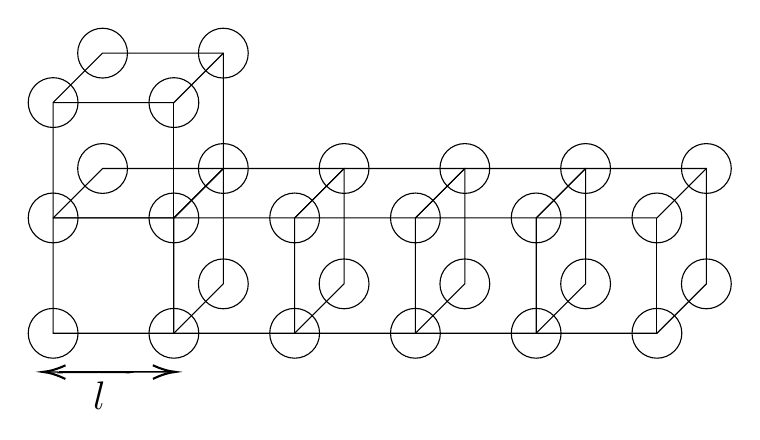
\begin{tikzpicture}[x=0.75pt,y=0.75pt,yscale=-1,xscale=1]
%uncomment if require: \path (0,300); %set diagram left start at 0, and has height of 300

%Shape: Cube [id:dp41969579234003374] 
\draw   (123,185.42) -- (146.82,161.6) -- (205,161.6) -- (205,217.18) -- (181.18,241) -- (123,241) -- cycle ; \draw   (205,161.6) -- (181.18,185.42) -- (123,185.42) ; \draw   (181.18,185.42) -- (181.18,241) ;
%Shape: Cube [id:dp8971766330143272] 
\draw   (181.18,185.42) -- (205,161.6) -- (263.18,161.6) -- (263.18,217.18) -- (239.36,241) -- (181.18,241) -- cycle ; \draw   (263.18,161.6) -- (239.36,185.42) -- (181.18,185.42) ; \draw   (239.36,185.42) -- (239.36,241) ;
%Shape: Cube [id:dp7065617623350473] 
\draw   (239.36,185.42) -- (263.18,161.6) -- (321.36,161.6) -- (321.36,217.18) -- (297.54,241) -- (239.36,241) -- cycle ; \draw   (321.36,161.6) -- (297.54,185.42) -- (239.36,185.42) ; \draw   (297.54,185.42) -- (297.54,241) ;
%Shape: Cube [id:dp03472830432500995] 
\draw   (297.54,185.42) -- (321.36,161.6) -- (379.54,161.6) -- (379.54,217.18) -- (355.72,241) -- (297.54,241) -- cycle ; \draw   (379.54,161.6) -- (355.72,185.42) -- (297.54,185.42) ; \draw   (355.72,185.42) -- (355.72,241) ;
%Shape: Cube [id:dp33777831467463404] 
\draw   (355.72,185.42) -- (379.54,161.6) -- (437.72,161.6) -- (437.72,217.18) -- (413.9,241) -- (355.72,241) -- cycle ; \draw   (437.72,161.6) -- (413.9,185.42) -- (355.72,185.42) ; \draw   (413.9,185.42) -- (413.9,241) ;
%Shape: Cube [id:dp47365929768009774] 
\draw   (123,129.84) -- (146.82,106.02) -- (205,106.02) -- (205,161.6) -- (181.18,185.42) -- (123,185.42) -- cycle ; \draw   (205,106.02) -- (181.18,129.84) -- (123,129.84) ; \draw   (181.18,129.84) -- (181.18,185.42) ;
%Shape: Circle [id:dp26181059419593056] 
\draw   (111,129.84) .. controls (111,123.21) and (116.37,117.84) .. (123,117.84) .. controls (129.63,117.84) and (135,123.21) .. (135,129.84) .. controls (135,136.47) and (129.63,141.84) .. (123,141.84) .. controls (116.37,141.84) and (111,136.47) .. (111,129.84) -- cycle ;
%Shape: Circle [id:dp9040339079317856] 
\draw   (169.18,129.84) .. controls (169.18,123.21) and (174.55,117.84) .. (181.18,117.84) .. controls (187.81,117.84) and (193.18,123.21) .. (193.18,129.84) .. controls (193.18,136.47) and (187.81,141.84) .. (181.18,141.84) .. controls (174.55,141.84) and (169.18,136.47) .. (169.18,129.84) -- cycle ;
%Shape: Circle [id:dp25927762994932513] 
\draw   (134.82,106.02) .. controls (134.82,99.39) and (140.19,94.02) .. (146.82,94.02) .. controls (153.45,94.02) and (158.82,99.39) .. (158.82,106.02) .. controls (158.82,112.65) and (153.45,118.02) .. (146.82,118.02) .. controls (140.19,118.02) and (134.82,112.65) .. (134.82,106.02) -- cycle ;
%Shape: Circle [id:dp06006139921847331] 
\draw   (193,106.02) .. controls (193,99.39) and (198.37,94.02) .. (205,94.02) .. controls (211.63,94.02) and (217,99.39) .. (217,106.02) .. controls (217,112.65) and (211.63,118.02) .. (205,118.02) .. controls (198.37,118.02) and (193,112.65) .. (193,106.02) -- cycle ;
%Shape: Circle [id:dp7364585134601493] 
\draw   (111,185.42) .. controls (111,178.79) and (116.37,173.42) .. (123,173.42) .. controls (129.63,173.42) and (135,178.79) .. (135,185.42) .. controls (135,192.05) and (129.63,197.42) .. (123,197.42) .. controls (116.37,197.42) and (111,192.05) .. (111,185.42) -- cycle ;
%Shape: Circle [id:dp7807195849394937] 
\draw   (169.18,185.42) .. controls (169.18,178.79) and (174.55,173.42) .. (181.18,173.42) .. controls (187.81,173.42) and (193.18,178.79) .. (193.18,185.42) .. controls (193.18,192.05) and (187.81,197.42) .. (181.18,197.42) .. controls (174.55,197.42) and (169.18,192.05) .. (169.18,185.42) -- cycle ;
%Shape: Circle [id:dp3602299886997964] 
\draw   (193,161.6) .. controls (193,154.97) and (198.37,149.6) .. (205,149.6) .. controls (211.63,149.6) and (217,154.97) .. (217,161.6) .. controls (217,168.23) and (211.63,173.6) .. (205,173.6) .. controls (198.37,173.6) and (193,168.23) .. (193,161.6) -- cycle ;
%Shape: Circle [id:dp041594438420205604] 
\draw   (309.36,161.6) .. controls (309.36,154.97) and (314.73,149.6) .. (321.36,149.6) .. controls (327.99,149.6) and (333.36,154.97) .. (333.36,161.6) .. controls (333.36,168.23) and (327.99,173.6) .. (321.36,173.6) .. controls (314.73,173.6) and (309.36,168.23) .. (309.36,161.6) -- cycle ;
%Shape: Circle [id:dp3778309487038063] 
\draw   (111,241) .. controls (111,234.37) and (116.37,229) .. (123,229) .. controls (129.63,229) and (135,234.37) .. (135,241) .. controls (135,247.63) and (129.63,253) .. (123,253) .. controls (116.37,253) and (111,247.63) .. (111,241) -- cycle ;
%Shape: Circle [id:dp6178134295790514] 
\draw   (251.18,161.6) .. controls (251.18,154.97) and (256.55,149.6) .. (263.18,149.6) .. controls (269.81,149.6) and (275.18,154.97) .. (275.18,161.6) .. controls (275.18,168.23) and (269.81,173.6) .. (263.18,173.6) .. controls (256.55,173.6) and (251.18,168.23) .. (251.18,161.6) -- cycle ;
%Shape: Circle [id:dp7457120548071341] 
\draw   (169.18,241) .. controls (169.18,234.37) and (174.55,229) .. (181.18,229) .. controls (187.81,229) and (193.18,234.37) .. (193.18,241) .. controls (193.18,247.63) and (187.81,253) .. (181.18,253) .. controls (174.55,253) and (169.18,247.63) .. (169.18,241) -- cycle ;
%Shape: Circle [id:dp1752040765903189] 
\draw   (193,217.18) .. controls (193,210.55) and (198.37,205.18) .. (205,205.18) .. controls (211.63,205.18) and (217,210.55) .. (217,217.18) .. controls (217,223.81) and (211.63,229.18) .. (205,229.18) .. controls (198.37,229.18) and (193,223.81) .. (193,217.18) -- cycle ;
%Shape: Circle [id:dp5389396478842299] 
\draw   (251.18,217.18) .. controls (251.18,210.55) and (256.55,205.18) .. (263.18,205.18) .. controls (269.81,205.18) and (275.18,210.55) .. (275.18,217.18) .. controls (275.18,223.81) and (269.81,229.18) .. (263.18,229.18) .. controls (256.55,229.18) and (251.18,223.81) .. (251.18,217.18) -- cycle ;
%Shape: Circle [id:dp11406795208586296] 
\draw   (227.36,185.42) .. controls (227.36,178.79) and (232.73,173.42) .. (239.36,173.42) .. controls (245.99,173.42) and (251.36,178.79) .. (251.36,185.42) .. controls (251.36,192.05) and (245.99,197.42) .. (239.36,197.42) .. controls (232.73,197.42) and (227.36,192.05) .. (227.36,185.42) -- cycle ;
%Shape: Circle [id:dp4825363325662064] 
\draw   (227.36,241) .. controls (227.36,234.37) and (232.73,229) .. (239.36,229) .. controls (245.99,229) and (251.36,234.37) .. (251.36,241) .. controls (251.36,247.63) and (245.99,253) .. (239.36,253) .. controls (232.73,253) and (227.36,247.63) .. (227.36,241) -- cycle ;
%Shape: Circle [id:dp7667565953901512] 
\draw   (134.82,161.6) .. controls (134.82,154.97) and (140.19,149.6) .. (146.82,149.6) .. controls (153.45,149.6) and (158.82,154.97) .. (158.82,161.6) .. controls (158.82,168.23) and (153.45,173.6) .. (146.82,173.6) .. controls (140.19,173.6) and (134.82,168.23) .. (134.82,161.6) -- cycle ;
%Shape: Circle [id:dp04333174499781589] 
\draw   (367.54,161.6) .. controls (367.54,154.97) and (372.91,149.6) .. (379.54,149.6) .. controls (386.17,149.6) and (391.54,154.97) .. (391.54,161.6) .. controls (391.54,168.23) and (386.17,173.6) .. (379.54,173.6) .. controls (372.91,173.6) and (367.54,168.23) .. (367.54,161.6) -- cycle ;
%Shape: Circle [id:dp13758925297473912] 
\draw   (309.36,217.18) .. controls (309.36,210.55) and (314.73,205.18) .. (321.36,205.18) .. controls (327.99,205.18) and (333.36,210.55) .. (333.36,217.18) .. controls (333.36,223.81) and (327.99,229.18) .. (321.36,229.18) .. controls (314.73,229.18) and (309.36,223.81) .. (309.36,217.18) -- cycle ;
%Shape: Circle [id:dp05424082814715736] 
\draw   (285.54,241) .. controls (285.54,234.37) and (290.91,229) .. (297.54,229) .. controls (304.17,229) and (309.54,234.37) .. (309.54,241) .. controls (309.54,247.63) and (304.17,253) .. (297.54,253) .. controls (290.91,253) and (285.54,247.63) .. (285.54,241) -- cycle ;
%Shape: Circle [id:dp6141763035080399] 
\draw   (343.72,241) .. controls (343.72,234.37) and (349.09,229) .. (355.72,229) .. controls (362.35,229) and (367.72,234.37) .. (367.72,241) .. controls (367.72,247.63) and (362.35,253) .. (355.72,253) .. controls (349.09,253) and (343.72,247.63) .. (343.72,241) -- cycle ;
%Shape: Circle [id:dp11138537616726163] 
\draw   (285.54,185.42) .. controls (285.54,178.79) and (290.91,173.42) .. (297.54,173.42) .. controls (304.17,173.42) and (309.54,178.79) .. (309.54,185.42) .. controls (309.54,192.05) and (304.17,197.42) .. (297.54,197.42) .. controls (290.91,197.42) and (285.54,192.05) .. (285.54,185.42) -- cycle ;
%Shape: Circle [id:dp2857114220838535] 
\draw   (343.72,185.42) .. controls (343.72,178.79) and (349.09,173.42) .. (355.72,173.42) .. controls (362.35,173.42) and (367.72,178.79) .. (367.72,185.42) .. controls (367.72,192.05) and (362.35,197.42) .. (355.72,197.42) .. controls (349.09,197.42) and (343.72,192.05) .. (343.72,185.42) -- cycle ;
%Shape: Circle [id:dp7714200384855789] 
\draw   (425.72,161.6) .. controls (425.72,154.97) and (431.09,149.6) .. (437.72,149.6) .. controls (444.35,149.6) and (449.72,154.97) .. (449.72,161.6) .. controls (449.72,168.23) and (444.35,173.6) .. (437.72,173.6) .. controls (431.09,173.6) and (425.72,168.23) .. (425.72,161.6) -- cycle ;
%Shape: Circle [id:dp3558846812341172] 
\draw   (401.9,185.42) .. controls (401.9,178.79) and (407.27,173.42) .. (413.9,173.42) .. controls (420.53,173.42) and (425.9,178.79) .. (425.9,185.42) .. controls (425.9,192.05) and (420.53,197.42) .. (413.9,197.42) .. controls (407.27,197.42) and (401.9,192.05) .. (401.9,185.42) -- cycle ;
%Shape: Circle [id:dp07542711406481573] 
\draw   (401.9,241) .. controls (401.9,234.37) and (407.27,229) .. (413.9,229) .. controls (420.53,229) and (425.9,234.37) .. (425.9,241) .. controls (425.9,247.63) and (420.53,253) .. (413.9,253) .. controls (407.27,253) and (401.9,247.63) .. (401.9,241) -- cycle ;
%Shape: Circle [id:dp3278021064225043] 
\draw   (425.72,217.18) .. controls (425.72,210.55) and (431.09,205.18) .. (437.72,205.18) .. controls (444.35,205.18) and (449.72,210.55) .. (449.72,217.18) .. controls (449.72,223.81) and (444.35,229.18) .. (437.72,229.18) .. controls (431.09,229.18) and (425.72,223.81) .. (425.72,217.18) -- cycle ;
%Straight Lines [id:da267643388635215] 
\draw    (126,259.6) -- (182,259.6) ;
%Straight Lines [id:da5500248139986914] 
\draw    (125,260) -- (180,259.61) ;
\draw [shift={(182,259.6)}, rotate = 179.6] [color={rgb, 255:red, 0; green, 0; blue, 0 }  ][line width=0.75]    (10.93,-3.29) .. controls (6.95,-1.4) and (3.31,-0.3) .. (0,0) .. controls (3.31,0.3) and (6.95,1.4) .. (10.93,3.29)   ;
%Straight Lines [id:da662294481940741] 
\draw    (160,260) -- (120,259.62) ;
\draw [shift={(118,259.6)}, rotate = 0.55] [color={rgb, 255:red, 0; green, 0; blue, 0 }  ][line width=0.75]    (10.93,-3.29) .. controls (6.95,-1.4) and (3.31,-0.3) .. (0,0) .. controls (3.31,0.3) and (6.95,1.4) .. (10.93,3.29)   ;
%Shape: Circle [id:dp8169223489901998] 
\draw   (367.54,217.18) .. controls (367.54,210.55) and (372.91,205.18) .. (379.54,205.18) .. controls (386.17,205.18) and (391.54,210.55) .. (391.54,217.18) .. controls (391.54,223.81) and (386.17,229.18) .. (379.54,229.18) .. controls (372.91,229.18) and (367.54,223.81) .. (367.54,217.18) -- cycle ;

% Text Node
\draw (141,263.2) node [anchor=north west][inner sep=0.75pt]  [font=\Large]  {$l$};


\end{tikzpicture}
\end{document}
%=============================================================================
% eof
%
% Local Variables:
% mode: latex
% mode: linum
% mode: auto-fill
% fill-column: 80
% TeX-master: t
% End:
